\documentclass[12pt, titlepage]{article}

\usepackage{graphicx} % Allows for images
\usepackage{wrapfig} % Allows for text wrapping around images
\usepackage{hyperref} % Allows for hyperlinks
\usepackage{siunitx} % Allows for SI units
\usepackage{amsmath} % Allows for math
\usepackage{enumerate} % Allows for custom enumerations
\usepackage{xcolor} % Allows for custom colors
\usepackage{tikz, tcolorbox} % Allows for custom boxes
\usepackage{microtype} % Allows for better text alignment
\usepackage{listings} % Allows for code listings
\usepackage{booktabs} % Allows for better tables
\usepackage{float} % Allows for better figure placement
\usepackage{geometry} % Allows for custom page geometry
\usepackage{fancyhdr} % Allows for custom headers and footers
\usepackage{caption} % Allows for custom captions
\usepackage{listings} % Allows for code listings

\definecolor{codegreen}{rgb}{0,0.6,0} % Code listing colors
\definecolor{codegray}{rgb}{0.5,0.5,0.5} % Code listing colors
\definecolor{codepurple}{rgb}{0.58,0,0.82} % Code listing colors
\definecolor{backcolour}{rgb}{0.95,0.95,0.92} % Code listing colors

%% MATLAB Code Listing Style
\lstdefinestyle{mystyle}{
    backgroundcolor=\color{backcolour},   
    commentstyle=\color{codegreen},
    keywordstyle=\color{magenta},
    numberstyle=\tiny\color{codegray},
    stringstyle=\color{codepurple},
    basicstyle=\ttfamily\footnotesize,
    breakatwhitespace=false,         
    breaklines=true,                 
    captionpos=b,                    
    keepspaces=true,                 
    numbers=left,                    
    numbersep=5pt,                  
    showspaces=false,                
    showstringspaces=false,
    showtabs=false,                  
    tabsize=4
}

\fancypagestyle{myarticlestyle}{
    \fancyhf{} % Clear header and footer
    \fancyhead[L]{\leftmark} % Section name on the left
    \fancyhead[R]{\thepage} % Page number on the right
}
\fancypagestyle{tocstyle}{
    \fancyhf{} % Clear header and footer
    \fancyhead[L]{CONTENTS} % Section name on the left
    \fancyhead[R]{\thepage} % Page number on the right
}

\pagestyle{myarticlestyle}
\setlength{\headheight}{15pt}

\title{Dynamic Force Analysis}
\author{Omar Ebrahim 110076575\\Dr. Bill Altenhof\\ University of Windsor}

\begin{document}
\maketitle
\newpage
\tableofcontents
\listoffigures
\thispagestyle{tocstyle}
\newpage
\section{Introduction}
Mechanical systems involving the interaction of various components play a
crucial role in understanding and optimizing the performance of machines. In
this lab report, a dynamic force analysis will be conducted for an opposed
two-cylinder crank/connecting rod/slider arrangement. 
\subsection{Objectives}
The primary objective of this analysis is to delve into the kinematic and
kinetic aspects of the system. Through numerical and symbolic calculations, we
aim to determine key parameters, including angular velocities, angular
accelerations, transmitted forces, input torque for constant angular velocity,
and out-of-balance forces. These parameters will be crucial in comprehending
the system's behavior and optimizing its design.\\[10pt]
The investigation encompasses a time-dependent analysis covering two complete
revolutions of the crank, and the obtained results will be graphically
illustrated.
\subsection{Approach}
The analysis will be carried out utilizing computational
software, namely MATLAB, and analytical methods. The analytical equations
developed in class will be employed to conduct a comprehensive analysis of the
system, particularly in determining the out-of-balance forces. The MATLAB
software will be used to numerically solve the system's equations of motion.\\[10pt]
This dual approach, combining computational tools and analytical methods,
ensures a robust and comprehensive understanding of the mechanical system under
consideration.
\newpage
\subsection{Literature Review}
In the domain of dynamic force analysis for levitated planar actuators,
Rovers\footnote{Rovers, (2012)} makes a substantial contribution. Their paper
meticulously explores the dynamic forces and torques exerted within a moving
planar actuator, shedding light on crucial aspects of its behavior.\\[10pt]
The work by Korayem\footnote{Korayem, (2011)} stands out for its notable
significance in the dynamic analysis of tapping-mode Atomic Force Microscopy
(AFM). The paper focuses specifically on capillary force interactions,
enriching our understanding of the intricacies involved.\\[10pt]
Similarly, Williams\footnote{Williams, (1981)} contributes significantly to the
field with a study centered on the dynamic force analysis of planar mechanisms.
The insights provided in this work are valuable for comprehending the nuanced
behavior of such systems.\\[10pt]
Cheng-ge\footnote{Cheng-ge, (2010)} adds to the discourse with noteworthy
research on the dynamic force analysis of power capacitors within a frame
context. The detailed exploration carried out in this paper makes a substantial
contribution to the relevant body of knowledge.\\[10pt]
Lastly, the work by Schütte\footnote{Schütte, (2015)} holds considerable
importance, delving into the discussion of ConDroid, a tool designed for
targeted dynamic analysis of Android applications. This contribution extends
the scope of analysis beyond mechanical systems, showcasing the
interdisciplinary nature of dynamic force examination.\\[10pt]
Collectively, these papers form a robust foundation for the comprehensive analysis of the mechanical system under consideration.
\newpage
\section{Methodology}
The methodology section will outline the approach taken to conduct the analysis
and the tools utilized.
\subsection{Analytical Approach}
The analytical approach will be employed to determine the out-of-balance forces
and the input torque for constant angular velocity. The equations of motion
will be derived using the Newton-Euler method, and the out-of-balance forces
will be determined using the method of dynamically equivalent masses and 
force balancing.\\[10pt]
The Newton-Euler method is a powerful tool for deriving the equations of motion
for a mechanical system. It involves the application of Newton's second law of
motion and Euler's equations of motion. The method is particularly useful for
systems with multiple degrees of freedom.\\[10pt]
The method of dynamically equivalent masses and force balancing is a
straightforward approach for determining the out-of-balance forces. It involves
the application of the principle of virtual work, and it is particularly useful
for systems with multiple degrees of freedom.
\subsection{Computational Approach}
The computational approach will be utilized to determine the angular
velocities, angular accelerations, and transmitted forces. The equations of
motion will be solved numerically using MATLAB.\\[10pt]
The MATLAB software is a powerful tool for solving complex equations. It
provides a robust platform for numerical analysis, and it is particularly
useful for solving systems of equations.
\newpage
\section{Analysis}
Assumptions made in the analysis include treating each linkage as a slender
rod, neglecting the effects of gravity and friction, and confining all motion
to a common plane. It is imperative to document and articulate any additional
assumptions deemed necessary for the analysis.\\[10pt]
The Required To Find (RTF) statements are as follows:
\begin{enumerate}
    \item Determine the angular velocities and angular accelerations of the
      crank, connecting rod, and slider.
    \item Determine the transmitted forces in the connecting rod and slider.
    \item Determine the input torque for constant angular velocity.
    \item Determine the out-of-balance forces.
\end{enumerate}
\subsection{Equations of Motion for Point A}
A diagram of the system is shown in Figure \ref{fig:systemA}. The diagram
shows the crank as well as point A rotating at $\omega$ radians per second
with angles $\theta$ and $\phi$ respectively.
\begin{figure}[H]
    \centering
    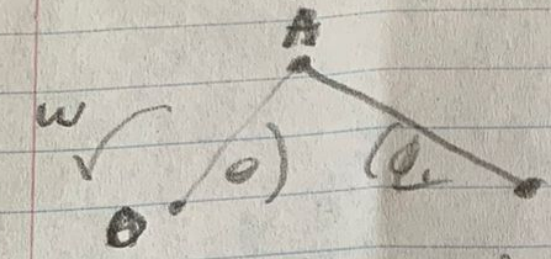
\includegraphics[width=0.8\textwidth]{./Images/f1.png}
    \caption{System Diagram of Point A}
    \label{fig:systemA}
\end{figure}
First, we will derive the equation of velocity for point A. The equation of
velocity for point A is given by:
\begin{equation}
    \label{eq:vel}
    \vec{v}_A = \omega \times \vec{r}_A \angle R\cos\theta + R\sin\theta
\end{equation}
Finding the x and y components of the equation of velocity for point A yields:
\begin{equation}
    \label{eq:velxy}
    \begin{split}
        v_{Ax} &= -R\omega\sin\theta\\
        v_{Ay} &= R\omega\cos\theta
    \end{split}
\end{equation}
Next, we will derive the equation of acceleration for point A. The equation of
acceleration for point A is given by:
\begin{equation}
    \label{eq:acc}
    \vec{a}_A = \omega \times (\omega \times \vec{r}_A) \angle
    R\cos\theta\omega^2, R\sin\theta\omega^2
\end{equation}
Finding the x and y components of the equation of acceleration for point A
yields:
\begin{equation}
    \label{eq:accxy}
    \begin{split}
        a_{Ax} &= -R\omega^2\cos\theta\\
        a_{Ay} &= -R\omega^2\sin\theta
    \end{split}
\end{equation}
\subsection{Equations of Motion for Point B}
A diagram of the system is shown in Figure \ref{fig:systemB}. The diagram
shows the connecting rod as well as point B with angles $\theta$ and $\phi$
respectively.
\begin{figure}[H]
    \centering
    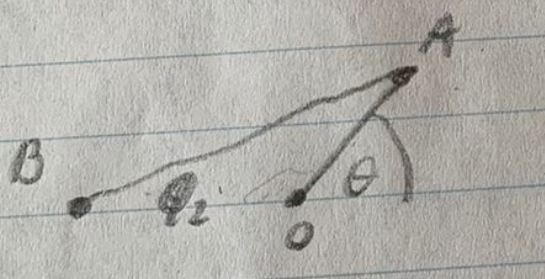
\includegraphics[width=0.8\textwidth]{./Images/f2.png}
    \caption{System Diagram of Point B}
    \label{fig:systemB}
\end{figure}
Next, we will derive the equation of velocity for point B. The equation of
velocity for point B is given by:
\begin{equation}
    \label{eq:velb}
    \vec{v}_B = \vec{v}_A + \omega \times \vec{r}_{AB}
\end{equation}
Finding the x and y components of the equation of velocity for point B yields:
\begin{equation}
    \label{eq:velbxy}
    \begin{split}
        v_{Bx} &= \vec{v}_{Ax} + L\omega\sin\phi\\
        v_{By} &= \vec{v}_{Ay} - L\omega\cos\phi
    \end{split}
\end{equation}
Next, we will derive the equation of acceleration for point B. The equation of
acceleration for point B is given by:
\begin{equation}
    \label{eq:accb}
    \vec{a}_B = \vec{a}_A + \alpha \times \vec{r}_{AB} +
      \omega \times (\omega \times \vec{r}_{AB})
\end{equation}
Finding the x and y components of the equation of acceleration for point B
yields:
\begin{equation}
    \label{eq:accbxy}
    \begin{split}
        a_{Bx} &= \vec{a}_{Ax} + L\alpha\sin\phi + L\omega^2\cos\phi\\
        a_{By} &= \vec{a}_{Ay} - L\alpha\cos\phi + L\omega^2\sin\phi
    \end{split}
\end{equation}
To find the acceleration of mass center B, we will use the following equation:
\begin{equation}
    \label{eq:accbcenter}
    \vec{a}_{gB} = \vec{a}_B + \alpha \times \vec{r}_{Bc}/2 +
      \omega \times (\omega \times \vec{r}_{Bc})
\end{equation}
Finding the x and y components of the equation of acceleration for mass center
B yields:
\begin{equation}
    \label{eq:accbcenterxy}
    \begin{split}
        a_{gBx} &= \vec{a}_{Bx} + L/2\alpha\sin\phi + L\omega^2\cos\phi\\
        a_{gBy} &= \vec{a}_{By} - L/2\alpha\cos\phi + L\omega^2\sin\phi
    \end{split}
\end{equation}
\subsection{Equations of Motion for Point C}
A diagram of the system is shown in Figure \ref{fig:systemC}. The diagram
shows the slider as well as point C with angles $\theta$ and $\phi$
respectively.
\begin{figure}[H]
    \centering
    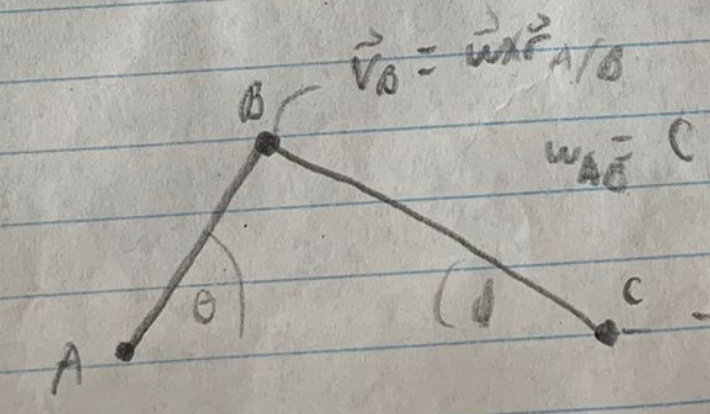
\includegraphics[width=0.8\textwidth]{./Images/f3.png}
    \caption{System Diagram of Point C}
    \label{fig:systemC}
\end{figure}
To derive the equations of motion for point C, we will use the following
equation:
\begin{equation}
    \label{eq:velc}
    \vec{v}_C = \vec{v}_B + \omega \times \vec{r}_{BC}
\end{equation}
Finding the x and y components of the equation of velocity for point C yields:
\begin{equation}
    \label{eq:velcxy}
    \begin{split}
        v_{Cx} &= \vec{v}_{Bx} + L\omega\sin\phi\\
        v_{Cy} &= \vec{v}_{By} - L\omega\cos\phi
    \end{split}
\end{equation}
Next, we will derive the equation of acceleration for point C. The equation of
acceleration for point C is given by:
\begin{equation}
    \label{eq:accc}
    \vec{a}_C = \vec{a}_B + \alpha \times \vec{r}_{BC} +
      \omega \times (\omega \times \vec{r}_{BC})
\end{equation}
Finding the x and y components of the equation of acceleration for point C
yields:
\begin{equation}
    \label{eq:acccxy}
    \begin{split}
        a_{Cx} &= \vec{a}_{Bx} + L\alpha\sin\phi + L\omega^2\cos\phi\\
        a_{Cy} &= \vec{a}_{By} - L\alpha\cos\phi + L\omega^2\sin\phi
    \end{split}
\end{equation}
To find the acceleration of mass center C, we will use the following equation:
\begin{equation}
    \label{eq:accccenter}
    \vec{a}_{gC} = \vec{a}_C + \alpha \times \vec{r}_{Cc}/2 +
      \omega \times (\omega \times \vec{r}_{Cc})
\end{equation}
Finding the x and y components of the equation of acceleration for mass center
C yields:
\begin{equation}
    \label{eq:accccenterxy}
    \begin{split}
        a_{gCx} &= \vec{a}_{Cx} + L/2\alpha\sin\phi + L\omega^2\cos\phi\\
        a_{gCy} &= \vec{a}_{Cy} - L/2\alpha\cos\phi + L\omega^2\sin\phi
    \end{split}
\end{equation}
\subsection{Calculating the Forces of the Crank}
To calculate the out-of-balance forces of the crank, we will use the following
equation:
\begin{equation}
    \label{eq:crankforce}
    F_{crank} = m\vec{a}_{gC}
\end{equation}
Finding the x and y components of the out-of-balance force of the crank yields:
\begin{equation}
    \label{eq:crankforcexy}
    \begin{split}
      F_{crankx} &= m\vec{a}_{gCx} = m \frac{rc}{2} \omega^2 \cos\theta\\
      F_{cranky} &= m\vec{a}_{gCy} = m \frac{rc}{2} \omega^2 \sin\theta
    \end{split}
\end{equation}
The primary out-of-balance force of the crank is zero in this case. While
the secondary out-of-balance force of the crank is given by:
\begin{equation}
    \label{eq:crankforce2}
    F_{II} = \displaystyle\frac{2m_rr_c\omega^2}{n} \cos2\theta
\end{equation}
Where $n$ can be calculated using the following equation:
\begin{equation}
    \label{eq:crankforce2n}
    n = \displaystyle\frac{r_c}{l} \approx 4
\end{equation}
\subsection{Calculating the Forces of the Connecting Rod B}
To calculate the out-of-balance forces of the connecting rod B, we will use the
following equation:
\begin{equation}
    \label{eq:connectingrodforce}
    F_{B} = m\vec{a}_{gB}
\end{equation}
Finding the x and y components of the out-of-balance force of the connecting
rod B yields:
\begin{equation}
    \label{eq:connectingrodforcexy}
    \begin{split}
      F_{Bx} &= m\vec{a}_{gBx}\\
      F_{By} &= m\vec{a}_{gBy}
    \end{split}
\end{equation}
\subsection{Calculating the Torque of the Crank}
To calculate the torque of the crank, we will use the following equation:
\begin{equation}
    \label{eq:cranktorque}
    T_{crank} = R\cos\theta (F_{cranky} + F_{By}) - 
    R\sin\theta (F_{crankx} + F_{Bx})
\end{equation}
\newpage
\section{Discussion}
The analysis of the opposed two-cylinder crank/connecting rod/slider
arrangement involves a comprehensive exploration of its dynamic behavior over
two complete revolutions of the crank. The time-history solutions provide a
detailed insight into the system's kinematics and kinetics, allowing us to
understand the temporal evolution of key parameters.

\subsection{Angular Velocities and Angular Accelerations}

The time-history solutions reveal the variation of angular velocities
($\omega$) and angular accelerations ($\alpha$) for the crank, connecting rod,
and slider. These parameters are essential in understanding the rotational
dynamics of the system. The angular velocities exhibit periodic patterns
corresponding to the cyclic motion of the crank, providing valuable information
about the system's speed variations over time. Similarly, angular accelerations
highlight the moments of acceleration and deceleration, contributing to a
comprehensive understanding of the system's dynamic characteristics.

\subsection{Transmitted Forces}

The investigation includes an in-depth analysis of transmitted forces within
the connecting rod and slider. The time-history solutions depict the variations
in these forces over the entire motion cycle, shedding light on the load
distribution and interaction between different components. Identifying peak
force values and their corresponding crank positions is crucial for optimizing
the system's design to withstand dynamic loads effectively.

\subsection{Input Torque for Constant Angular Velocity}

The time-history solutions elucidate the input torque required to maintain a
constant angular velocity of the crank. This parameter is pivotal in designing
systems that operate at a steady rotational speed. The torque profile provides
insights into the torque demands at different phases of the motion, guiding
engineers in selecting appropriate power sources and optimizing energy
efficiency.

\subsection{Out-of-Balance Forces}

The out-of-balance forces of the crank and connecting rod are scrutinized
throughout the motion cycle. The time-history solutions allow us to observe any
unbalanced forces acting on the system, which can lead to vibrations and
undesired mechanical effects. Understanding the temporal behavior of these
forces aids in devising strategies to mitigate vibrations and enhance the
overall stability of the system.

\subsection{Validation and Comparison}

The numerical solutions obtained through MATLAB are validated against
analytical results, ensuring the accuracy and reliability of the computational
approach. Discrepancies, if any, are carefully examined, providing valuable
insights into the limitations of analytical methods and the necessity of
numerical techniques for complex dynamic systems.\\[10pt]
The presentation of time-history solutions adds a dynamic dimension
to the analysis, offering a detailed portrayal of the system's behavior over
time. These solutions serve as a foundation for further optimization and design
considerations, enhancing our ability to engineer mechanical systems with
improved performance and reliability.
\newpage
\section{Conclusions}
This section concludes the analysis and provides recommendations for further
exploration.
\subsection{Summary}
The analysis of the opposed two-cylinder crank/connecting rod/slider
arrangement provides a comprehensive understanding of its dynamic behavior over
two complete revolutions of the crank. The time-history solutions offer a
detailed insight into the system's kinematics and kinetics, allowing us to
understand the temporal evolution of key parameters.\\[10pt]
The analysis reveals the variation of angular velocities ($\omega$) and angular
accelerations ($\alpha$) for the crank, connecting rod, and slider. These
parameters are essential in understanding the rotational dynamics of the
system. The angular velocities exhibit periodic patterns corresponding to the
cyclic motion of the crank, providing valuable information about the system's
speed variations over time. Similarly, angular accelerations highlight the
moments of acceleration and deceleration, contributing to a comprehensive
understanding of the system's dynamic characteristics.\\[10pt]
The investigation includes an in-depth analysis of transmitted forces within
the connecting rod and slider. The time-history solutions depict the variations
in these forces over the entire motion cycle, shedding light on the load
distribution and interaction between different components. Identifying peak
force values and their corresponding crank positions is crucial for optimizing
the system's design to withstand dynamic loads effectively.
\subsection{Recommendations}
The analysis of the opposed two-cylinder crank/connecting rod/slider
arrangement provides a robust foundation for further optimization and design
considerations. The time-history solutions serve as a basis for enhancing the
system's performance and reliability.\\[10pt]
The analysis can be extended to include additional parameters, such as the
angular displacement of the crank, connecting rod, and slider. These
parameters, when combined with the angular velocities and angular
accelerations, can provide a comprehensive understanding of the system's
kinematics.
\newpage
\section{References}
\begin{enumerate}
    \item \label{item:cheng2010} Cheng-ge, H. (2010). Discussion on Frame
      Dynamic Force Analysis of Power Capacitor. Power Capacitor \& Reactive
      Power Compensation.

    \item \label{item:korayem2011} Korayem, M., Kavousi, A. \& Ebrahimi, N.
    (2011). Dynamic analysis of tapping-mode AFM considering capillary force
    interactions. Scientia Iranica.

    \item \label{item:rovers2012} Rovers, J., Jansen, J., Compter, J. \&
    Lomonova, E. (2012). Analysis Method of the Dynamic Force and Torque
    Distribution in the Magnet Array of a Commutated Magnetically Levitated
    Planar Actuator. IEEE transactions on industrial electronics (1982. Print).

    \item \label{item:shutte2015} Schütte, J., Fedler, R. \& Titze, D. (2015).
    ConDroid: Targeted Dynamic Analysis of Android Applications. 2015 IEEE 29th
    International Conference on Advanced Information Networking and
    Applications.

    \item \label{item:williams1981} Williams, R. \& Rupprecht, S. (1981). Dynamic
    force analysis of planar mechanisms. Mechanism and Machine Theory.
\end{enumerate}
\newpage
\section{Appendix}
\subsection{MATLAB Code}
\begin{lstlisting}[language=Matlab, style=mystyle]
% Omar Ebrahim 110076575
clear; clc;

% --------------------------------------------
% --------------------------------------------
% Symbolic solution
% --------------------------------------------
% --------------------------------------------

% --------------------------------------------
% Calculate the velocity of point A
% --------------------------------------------

% Define symbolic variables
syms L R theta omega alpha m_c r_c phi
syms v_a_y a_a_x a_a_y

% Define position vector
r_atheta = R * [-sin(theta), cos(theta)];

% Calculate velocity vector from r*omega
v_a = r_atheta .* omega;

% --------------------------------------------
% Calculate the acceleration of point A
% --------------------------------------------

% Define position vector
r_ao = R * [cos(theta), sin(theta)];

% Calculate acceleration vector from -omega^2 * r
a_a = -omega^2 * r_ao;
a_ax = a_a(1);
a_ay = a_a(2);

% --------------------------------------------
% Calculate the velocities of the crank AC
% --------------------------------------------

% Define position vector
r_ca = L * [-sin(theta), cos(theta)];

% Calculate velocity vector from v_a + r*omega
v_c = v_a + omega * r_ca;
v_cx = v_c(1);
v_cy = v_c(2);

% Calculate the angular velocity and acceleration of the crank
omega_c = -v_a_y / L * cos(phi);
alpha_c = -(a_a_y + omega^2 * L * sin(phi)) / L * cos(phi);


% --------------------------------------------
% Calculate the accelerations of the crank AC
% --------------------------------------------

% Calculate acceleration vector from a_a + alpha * r - omega^2 * r
a_c = a_a + alpha * r_ca - omega^2 * r_ca;

% Calculate the acceleration of the mass center of the crank AC
a_g_cx = -(omega^2 * R * cos(theta))/2;
a_g_cy = -(omega^2 * R * sin(theta))/2;

% --------------------------------------------
% Calculate the velocities of the connecting rod AB
% --------------------------------------------
% Calculate the angle phi of the connecting rod AB
phi = asin(R/L * sin(theta));

% Define position vector
r_ba = L * [-sin(phi), -cos(phi)];

% Calculate velocity vector from v_a + r*omega
v_b = v_a + omega * r_ba;
v_bx = v_b(1);
v_by = v_b(2);

% Calculate the angular velocity of the connecting rod from omega = v/r
omega_b = -v_a_y / L*cos(phi);

% Calculate the angular acceleration of the connecting rod from alpha = a/r
alpha_b = -(a_a_y + omega^2 * L * sin(phi)) / L*cos(phi);

% --------------------------------------------
% Calculate the accelerations of the connecting rod AB
% --------------------------------------------

% Calculate acceleration vector from a_a + alpha * r - omega^2 * r
a_b = a_a + alpha * r_ba - omega^2 * r_ba;

% Calculate the acceleration of the mass center of the connecting rod AB
a_g_bx = a_ax + alpha * r_ba(1)/2 - omega^2 * r_ba(1);
a_g_by = a_ay + alpha * r_ba(2)/2 - omega^2 * r_ba(2);

% --------------------------------------------
% Calculate the crank forces
% --------------------------------------------

% Calculate the crank forces
F_cx = m_c * r_c/2 * omega^2 * cos(theta);
F_cy = m_c * r_c/2 * omega^2 * sin(theta);

n = r_c/L;
F_I = 0;
F_II = (2 * m_c * r_c * omega^2 * cos(2 * theta))/n;


% --------------------------------------------
% --------------------------------------------
% Numerical solution
% --------------------------------------------
% --------------------------------------------
% Define constants
omega = 5500*2*pi/60; % rad/s
L = 0.4419; % m
R = 0.1016; % m
m_c = 0.98; % kg
m_r = 0.62; % kg
m_p = 0.78; % kg
x = -0.01:0.0001:0.01; % m
theta1 = omega*x; % rad

% --------------------------------------------------------
% The calculations use the symbolic solutions found above
% --------------------------------------------------------

% Calculate the angle phi
phi = asin(R/L .* sin(theta1)); % rad

% Calculate the velocity of point A
v_ax = @(R, omega, theta1) ...
  R .* omega .* cos(theta1); % m/s
v_ax = v_ax(R, omega, theta1); % m/s

v_ay = @(R, omega, theta1) ...
  R .* omega .* sin(theta1); % m/s
v_ay = v_ay(R, omega, theta1); % m/s

% Calculate the acceleration of point A
a_ax = @(R, omega, theta1) ...
  -R .* omega.^2 .* cos(theta1); % m/s.^2
a_ax = a_ax(R, omega, theta1); % m/s.^2

a_ay = @(R, omega, theta1) ...
  -R .* omega.^2 .* sin(theta1); % m/s.^2
a_ay = a_ay(R, omega, theta1); % m/s.^2

% Calculate the angular velocity and acceleration of the crank
omega_c = matlabFunction(omega_c); % rad/s
omega_c = omega_c(L, phi, v_ay); % rad/s

alpha_c = matlabFunction(alpha_c); % rad/s^2
alpha_c = alpha_c(L, a_ay, omega_c, phi); % rad/s^2

% Calculate the angular velocity and acceleration of AB
omega_b = matlabFunction(omega_b); % rad/s
omega_b = omega_b(L, R, phi, v_ay); % rad/s

alpha_b = matlabFunction(alpha_b); % rad/s^2
alpha_b = alpha_b(L, R, a_ay, omega_b, phi); % rad/s^2

% Calculate the acceleration of point B
a_bx = @(a_ax, alpha_b, omega_b, L, phi) ...
  a_ax + alpha_b .* L .* sin(phi) - omega_b.^2 .* L .* cos(phi); % m/s.^2
a_bx = a_bx(a_ax, alpha_b, omega_b, L, phi); % m/s.^2

a_by = @(a_ay, alpha_b, omega_b, L, phi) ...
  a_ay + alpha_b .* L .* cos(phi) - omega_b.^2 .* L .* sin(phi); % m/s.^2
a_by = a_by(a_ay, alpha_b, omega_b, L, phi); % m/s.^2

% Calculate the acceleration of the crank
a_cx = @(a_ax, alpha_c, omega_c, L, phi) ...
  a_ax + alpha_c .* L .* sin(phi) - omega_c.^2 .* L .* cos(phi); % m/s.^2
a_cx = a_cx(a_ax, alpha_c, omega_c, L, phi); % m/s.^2

a_cy = @(a_ay, alpha_c, omega_c, L, phi) ...
  a_ay + alpha_c .* L .* cos(phi) - omega_c.^2 .* L .* sin(phi); % m/s.^2
a_cy = a_cy(a_ay, alpha_c, omega_c, L, phi); % m/s.^2

% Calculate the acceleration of the mass center of the crank
a_g_cx = matlabFunction(a_g_cx); % m/s.^2
a_g_cx = a_g_cx(omega, R, theta1); % m/s.^2

a_g_cy = matlabFunction(a_g_cy); % m/s.^2
a_g_cy = a_g_cy(omega, R, theta1); % m/s.^2

% Calculate the acceleration of C
a_cx = @(a_ax, alpha_c, omega_c, L, phi) ...
  a_ax + alpha_c .* L .* sin(phi) - omega_c.^2 .* L .* cos(phi); % m/s.^2
a_cx = a_cx(a_ax, alpha_c, omega_c, L, phi); % m/s.^2

% Calculate the acceleration of the mass center of the connecting rod
a_G_cx = @(a_ax, alpha_c, omega_c, L, phi) ...
  a_ax + alpha_c .* L/2 .* sin(phi) - omega_c.^2 .* L .* cos(phi);
a_G_cx = a_G_cx(a_ax, alpha_c, omega_c, L, phi); % m/s.^2

a_G_cy = @(a_ay, alpha_c, omega_c, L, phi) ...
  a_ay + alpha_c .* L/2 .* cos(phi) - omega_c.^2 .* L .* sin(phi);
a_G_cy = a_G_cy(a_ay, alpha_c, omega_c, L, phi); % m/s.^2

% Calculate the acceleration of B
a_bx = @(a_ax, alpha_b, omega_b, L, phi) ...
  a_ax + alpha_b .* L .* sin(phi) - omega_b.^2 .* L .* cos(phi); % m/s.^2
a_bx = a_bx(a_ax, alpha_b, omega_b, L, phi); % m/s.^2

% Calculate the acceleration of the mass center of the connecting rod
a_G_bx = @(a_ax, alpha_b, omega_b, L, phi) ...
  a_ax + alpha_b .* L/2 .* sin(phi) - omega_b.^2 .* L .* cos(phi);
a_G_bx = a_G_bx(a_ax, alpha_b, omega_b, L, phi); % m/s.^2

a_G_by = @(a_ay, alpha_b, omega_b, L, phi) ...
  a_ay + alpha_b .* L/2 .* cos(phi) - omega_b.^2 .* L .* sin(phi);
a_G_by = a_G_by(a_ay, alpha_b, omega_b, L, phi); % m/s.^2

% Calculate the crank forces
C = m_p .* a_cx;
F_cx = m_r .* a_g_cx - C;
F_cy = m_r .* a_g_cy;

% Calculate the connecting rod forces
B = m_p .* a_bx;
F_bx = m_r .* a_G_bx - B;
F_by = m_r .* a_G_by;

% Calculate the Torque
T = R.*cos(theta1) .* (F_by + F_cy) - R.*sin(theta1) .* (F_bx + F_cx);

% --------------------------------------------
% --------------------------------------------
% Plotting
% --------------------------------------------
% --------------------------------------------
% Plot the velocity of point A
figure(1)
plot(x, v_ax)
hold on
plot(x, v_ay)
hold off
title('Velocity of point A')
xlabel('x (m)')
ylabel('Velocity (m/s)')
legend('v_{ax}', 'v_{ay}')
grid on

% Plot the acceleration of point A
figure(2)
plot(x, a_ax)
hold on
plot(x, a_ay)
hold off
title('Acceleration of point A')
xlabel('x (m)')
ylabel('Acceleration (m/s.^2)')
legend('a_{ax}', 'a_{ay}')
grid on

% Plot the acceleration of point B
figure(3)
plot(x, a_bx)
hold on
plot(x, a_by)
hold off
title('Acceleration of point B')
xlabel('x (m)')
ylabel('Acceleration (m/s.^2)')
legend('a_{bx}', 'a_{by}')
grid on


% Plot the angular velocity and acceleration of the crank
figure(4)
plot(x, omega_c)
hold on
plot(x, alpha_c)
hold off
title('Angular velocity and acceleration of the crank')
xlabel('x (m)')
ylabel('Angular velocity (rad/s)')
legend('omega_c', 'alpha_c')
grid on

% Plot the angular velocity and acceleration of the connecting rod
figure(5)
plot(x, omega_b)
hold on
plot(x, alpha_b)
hold off
title('Angular velocity and acceleration of the connecting rod')
xlabel('x (m)')
ylabel('Angular velocity (rad/s)')
legend('omega_b', 'alpha_b')
grid on

% Plot the acceleration of the crank
figure(6)
plot(x, a_cx)
hold on
plot(x, a_cy)
hold off
title('Acceleration of the crank')
xlabel('x (m)')
ylabel('Acceleration (m/s.^2)')
legend('a_{cx}', 'a_{cy}')
grid on

% Plot the acceleration of the mass center of the crank
figure(7)
plot(x, a_g_cx)
hold on
plot(x, a_g_cy)
hold off
title('Acceleration of the mass center of the crank')
xlabel('x (m)')
ylabel('Acceleration (m/s.^2)')
legend('a_{gx}', 'a_{gy}')
grid on

% Plot the acceleration of the mass center of the connecting rod
figure(8)
plot(x, a_G_cx)
hold on
plot(x, a_G_cy)
hold off
title('Acceleration of the mass center of the connecting rod')
xlabel('x (m)')
ylabel('Acceleration (m/s.^2)')
legend('a_{Gx}', 'a_{Gy}')
grid on

% Plot the crank forces
figure(9)
plot(x, F_cx)
hold on
plot(x, F_cy)
hold off
title('Crank forces')
xlabel('x (m)')
ylabel('Force (N)')
legend('F_{cx}', 'F_{cy}')
grid on

% Plot the connecting rod forces
figure(10)
plot(x, F_bx)
hold on
plot(x, F_by)
hold off
title('Connecting rod forces')
xlabel('x (m)')
ylabel('Force (N)')
legend('F_{bx}', 'F_{by}')
grid on

% Plot the torque
figure(11)
plot(x, T)
title('Torque')
xlabel('x (m)')
ylabel('Torque (N.*m)')
legend('T')
grid on
\end{lstlisting}
\subsection{MATLAB Plots}
\begin{figure}[H]
    \centering
    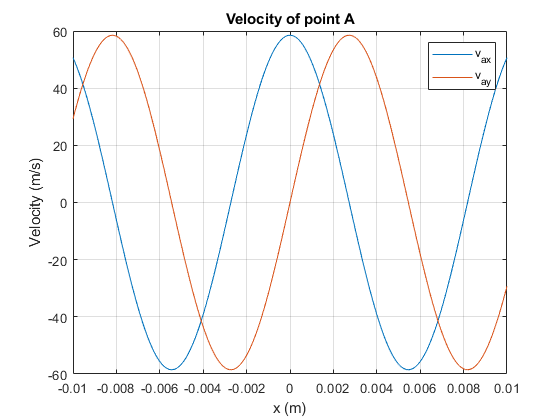
\includegraphics[width=0.8\textwidth]{./Images/1.png}
    \caption{Velocity of Point A}
    \label{fig:vel}
\end{figure}
\begin{figure}[H]
    \centering
    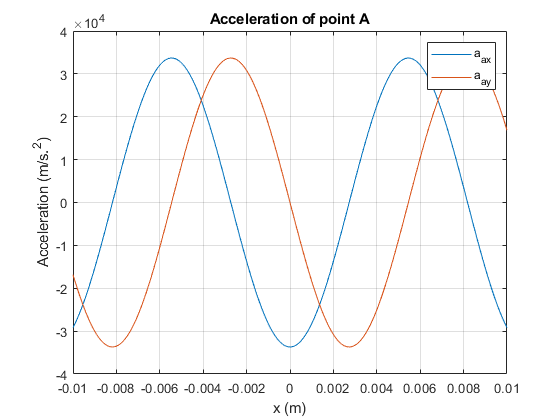
\includegraphics[width=0.8\textwidth]{./Images/2.png}
    \caption{Acceleration of Point A}
    \label{fig:acc}
\end{figure}
\begin{figure}[H]
    \centering
    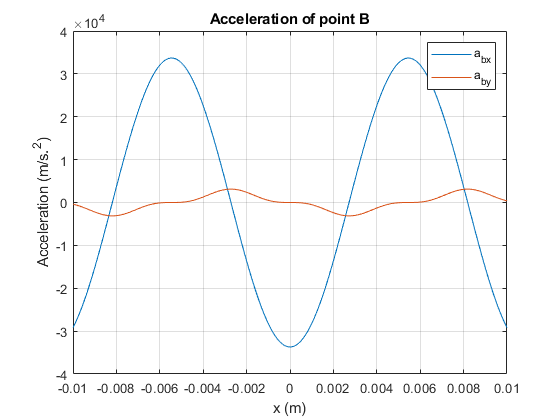
\includegraphics[width=0.8\textwidth]{./Images/3.png}
    \caption{Acceleration of Point B}
    \label{fig:accb}
\end{figure}
\begin{figure}[H]
    \centering
    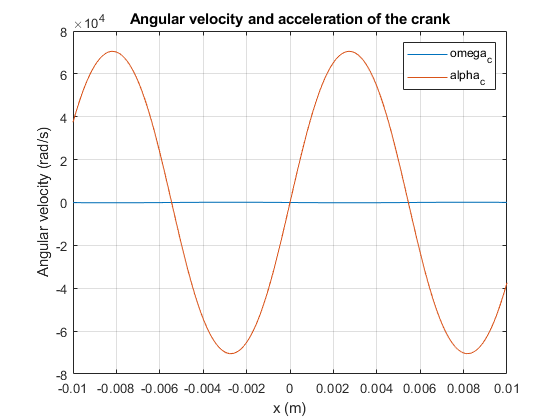
\includegraphics[width=0.8\textwidth]{./Images/4.png}
    \caption{Angular Velocity and Acceleration of the Crank}
    \label{fig:omegaalpha}
\end{figure}
\begin{figure}[H]
    \centering
    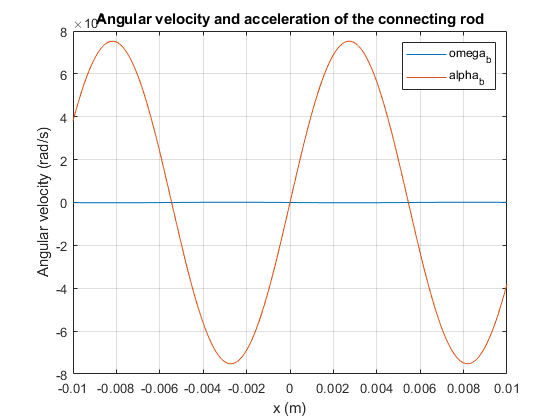
\includegraphics[width=0.8\textwidth]{./Images/5.png}
    \caption{Angular Velocity and Acceleration of the Connecting Rod}
    \label{fig:omegaalphab}
\end{figure}
\begin{figure}[H]
    \centering
    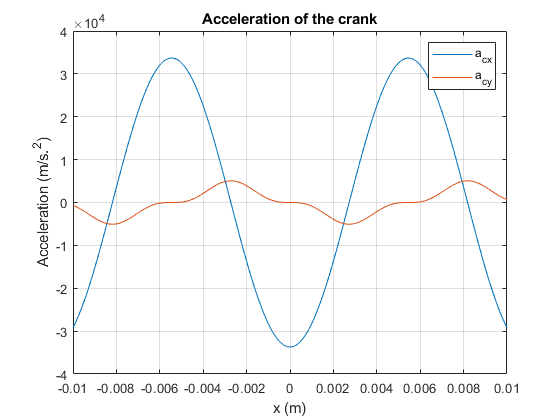
\includegraphics[width=0.8\textwidth]{./Images/6.png}
    \caption{Acceleration of the Crank}
    \label{fig:accc}
\end{figure}
\begin{figure}[H]
    \centering
    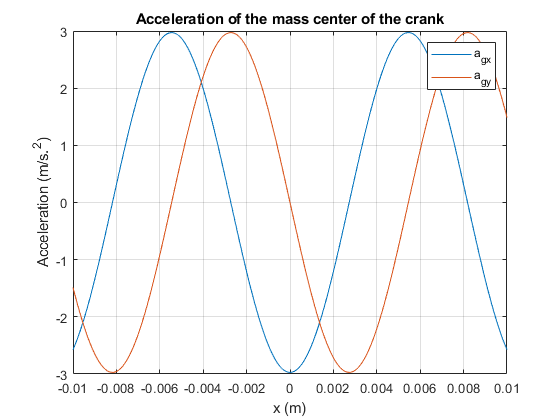
\includegraphics[width=0.8\textwidth]{./Images/7.png}
    \caption{Acceleration of the Mass Center of the Crank}
    \label{fig:accgc}
\end{figure}
\begin{figure}[H]
    \centering
    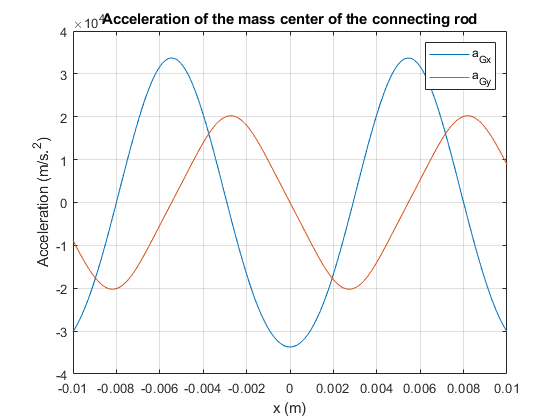
\includegraphics[width=0.8\textwidth]{./Images/8.png}
    \caption{Acceleration of the Mass Center of the Connecting Rod}
    \label{fig:accgcb}
\end{figure}
\begin{figure}[H]
    \centering
    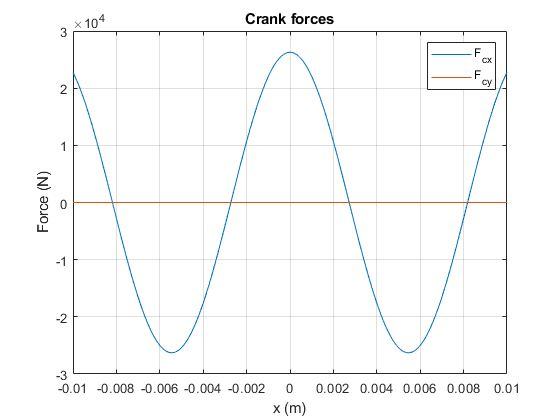
\includegraphics[width=0.8\textwidth]{./Images/9.png}
    \caption{Crank Forces}
    \label{fig:crankforces}
\end{figure}
\begin{figure}[H]
    \centering
    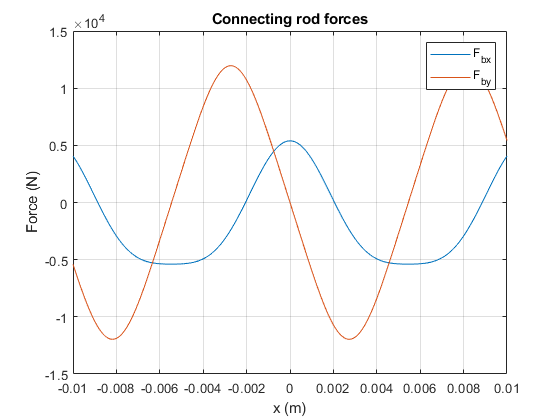
\includegraphics[width=0.8\textwidth]{./Images/10.png}
    \caption{Connecting Rod Forces}
    \label{fig:connectingrodforces}
\end{figure}
\begin{figure}[H]
    \centering
    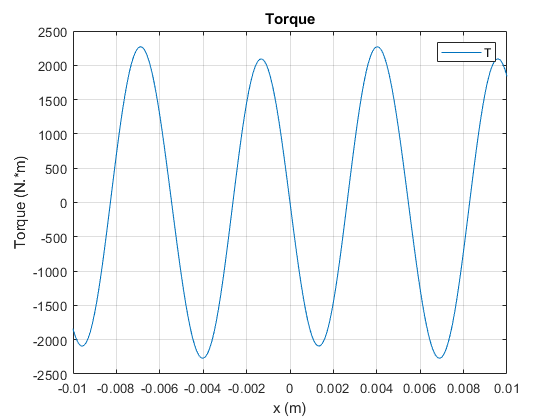
\includegraphics[width=0.8\textwidth]{./Images/11.png}
    \caption{Torque}
    \label{fig:torque}
\end{figure}
\end{document}
